\setchapterpreamble[u]{\margintoc}

\chapter{Homología de las superficies compactas}
Según el teorema de clasificación de superficies compactas, toda superficie
compacta y conexa es homeomorfa a $S^2$, a la suma conexa de $n$ toros o a la
suma conexa de $n$ planos proyectivos. Entre otras cosas, eso hace que las
componentes conexas de una superficie sean arcoconexas, dado que la
arcoconexión es una propiedad topológica.

Si llamamos $S_1,\dots,S_n$ a las componentes conexas de $S$, se tiene que
\[H_*(S)\cong \sum^n_{i=1}H_*(S_i)\]
por lo que podemos suponer a efectos de homología que $S$ es arcoconexa.

Por limitaciones de tiempo, nos restringiremos al caso de las superficies
orientables, que es más breve.

\subsection{Homología del $n$-toro}
\marginnote[-2.2cm]{
\begin{kaobox}[frametitle=Suma conexa de variedades]
Sea $X$ un espacio topológico Hausdorff y 2AN. Decimos que $X$ es una
$n$-variedad si, dado $p \in X$, existe un entorno abierto $U \subset X$ de
$p$ que sea homeomorfo a una bola abierta de $\mb{R}^n$.
Dadas dos $n$-variedades $X$ e $Y$, la suma conexa se define como
\[X\#Y=(X\backslash U)\cup_f (Y\backslash V)\]
siendo $U\subset X$, $V \subset Y$ abiertos y $f\colon \p U \to \p V$ continua.
\end{kaobox}
}
El $n$-toro (que denotaremos como $T_n$) se define como la suma conexa de $n$
toros. Podemos hacer la suma conexa de los representantes llanos, en cuyo caso
obtenemos una superficie como la que se puede ver en la \reffig{Bitoro}.

Si eliminamos el interior de $T_n$, la figura resultante será $B^1_{2n}$.  Si
$\gamma(t)=e^{2\pi i\theta}$, consideramos una aplicación $f\colon S^1\to
B_{2n}^1$ tal que
\[c_j=(f\circ\gamma)\left(\frac{j-1}{2n},\frac{j}{2n}\right)\]
es igual a cada uno de los pétalos de $B^1_{2n}$, con $j=1,\dots,2n$. Tenemos
entonces que $T_n=(B_{2n})_f$ (ver \reffig{Bitoro}). 

\marginnote[-2.2cm]{
\begin{kaobox}[frametitle=Ejercicio]
Comprueba que la cadena singular $c$ que estamos definiendo verifica que
$f([c])=0$ para $n=1,2,3$. Para $n=2$, puedes usar la \reffig{Bitoro} como
referencia; para $n=1,3$, es bueno dibujar el $n$-toro llano correspondiente.
\end{kaobox}
}

Vamos a estudiar la aplicación $f_*: \tilde{H}_1(S^1) \to H_1(B^1_{2n})$. El
grupo $\tilde{H}_1(S^1)$ tiene un único generador, $[c]$. Como representante
$c$, podemos elegir cualquier camino que dé una vuelta completa a $S^1$ (si no
da una vuelta completa, lo podemos contraer en un punto, por lo que está en la
clase del $0$). En particular, podemos elegir
\[c=\phi_1+\phi_2-(\phi_3+\phi_4)+\dots...+
	\phi_{2n-3}+\phi_{2n-2}-(\phi_{2n-1}+\phi_{2n})\]
donde $\phi_j(\sigma_1)=c_j$. Esta elección verifica que $f([c])=0$. Por tanto,
\begin{align*}
\im f_*=\{0\}; && \ker f_*=\tilde H_1(S^1)\cong \mb{Z}
\end{align*}

Por la proposición \refprop{CWHomo}, $H_p(T_n)\cong H_p(B^1_{2n})=0$ para todo
$p > 2$ y $H_1(T_n) \cong H_1(B_{2n})\cong \mb{Z}^{2n}$. Sólo nos queda
calcular el grupo de homología de orden 2:
\[0 \longrightarrow H_2(B^1_{2n}) \longrightarrow H_2(T_n) \longrightarrow
\tilde{H}_1(S^1) \longrightarrow 0\]
Dado que $H_2(B^1_{2n})=0$, se tiene por exactitud que
\[H_2(T_n) \cong \tilde{H}_1(S^1) \cong \mb{Z}\]

\begin{marginfigure}
\resizebox{\textwidth}{!}{
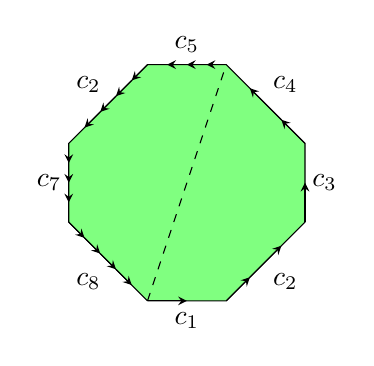
\begin{tikzpicture}
%Octógono
\draw[fill=green!50] (1,0) -- (2,0) -- (3,1) -- (3,2) -- (2,3) --
				(1,3) -- (0,2) -- (0,1) -- (1,0);

%La línea a través de la cual hacemos la suma conexa
\draw[dashed] (1,0) -- (2,3);

%Identificación de los lados
%c1
\draw[-stealth] (1,0) -- (1.5,0);
\draw (1.5,-.25) node {$c_1$};

%c2
\draw[-stealth] (2,0) -- (2.3,.3);
\draw[-stealth] (2.3,.3) -- (2.7,.7);
\draw (2.75,.25) node {$c_2$};

%c3
\draw[-stealth] (3,1) -- (3,1.5);
\draw (3.25,1.5) node {$c_3$};

%c4
\draw[-stealth] (3,2) -- (2.7,2.3);
\draw[-stealth] (2.7,2.3) -- (2.3,2.7);
\draw (2.75,2.75) node {$c_4$};

%c5
\draw[-stealth] (2,3) -- (1.75,3);
\draw[-stealth] (1.75,3) -- (1.5,3);
\draw[-stealth] (1.5,3) -- (1.25,3);
\draw (1.5,3.25) node {$c_5$};

%c6
\draw[-stealth] (1,3) -- (.8,2.8);
\draw[-stealth] (.8,2.8) -- (.6,2.6);
\draw[-stealth] (.6,2.6) -- (.4,2.4);
\draw[-stealth] (.4,2.4) -- (.2,2.2);
\draw (.25,2.75) node {$c_2$};

%c7
\draw[-stealth] (0,2) -- (0,1.75);
\draw[-stealth] (0,1.75) -- (0,1.5);
\draw[-stealth] (0,1.5) -- (0,1.25);
\draw (-.25,1.5) node {$c_7$};

%c8
\draw[-stealth] (0,1) -- (.2,.8);
\draw[-stealth] (.2,.8) -- (.4,.6);
\draw[-stealth] (.4,.6) -- (.6,.4);
\draw[-stealth] (.6,.4) -- (.8,.2);
\draw (.25,.25) node {$c_8$};
\end{tikzpicture}
}
\resizebox{\textwidth}{!}{
\begin{tikzpicture}
\draw[fill=green!50] (0,0) -- (0,2) -- (2,2) -- (2,0) -- (0,0);
\draw[dashed] (1,2) -- (2,1);
\draw (1,1) node {$T_1$};
\draw (2.3,1.5) node {$U$};

\draw[fill=green!50] (4,0) -- (4,2) -- (6,2) -- (6,0) -- (4,0);
\draw[dashed] (4,1) -- (5,2);
\draw (5,1) node {$T_1$};
\draw (3.7,1.5) node {$V$};

\begin{scope}
\clip (1,2) -- (5,2) -- (4,1) -- (2,1) -- (1,2);
\draw[pattern=north east lines] (1,1) -- (1,2) -- (2,2) -- (2,1) -- cycle;
\draw[pattern=north west lines] (4,1) -- (4,2) -- (6,2) -- (6,1) -- cycle;
\end{scope}

\draw[-stealth] (1.5,2.25) .. controls (2.5,2.75) and (3.5,2.75) .. (4.5,2.25);
\draw (3,2.25) node {$f$};
\end{tikzpicture}
}
\caption[Bitoro llano.]{\labfig{Bitoro} Bitoro llano. Los lados con el mismo
número de cabezas de flecha se identifican entre sí. La línea discontinua
separa los dos toros que lo conforman.}
\end{marginfigure}

De esta forma, \[H_n(T_n)\cong
\begin{cases}
\mb{Z}^{2n}	&\text{ si $n =1$}\\
\mb{Z}		&\text{ si $n=0,2$}\\
0			&\text{ si no}
\end{cases}\]

\begin{theorem}
Sea $S$ una superficie compacta y orientable con $\alpha$ componentes
conexas. Existe un $n \geq 0$ tal que
\[H_q(S)\cong \begin{cases}
\mb{Z}^{2n\alpha}	&\text{ si $q =1$}\\
\mb{Z}^\alpha		&\text{ si $q =0,2$}\\
0   				&\text{ si no}
\end{cases}\]
El valor $n$ se denomina \textbf{género} de la superficie.
\end{theorem}

\subsection{Espacio proyectivo real}
\begin{definition}
Dados $v,w \in S^n$, diremos que $v \sim w$ si $w=\pm v$. Definimos el espacio
proyectivo real $\mb{R}P^n$ como el cociente $S^n/\sim$.
\end{definition}

El espacio proyectivo real se puede entender como el espacio topológico
cuyos puntos son las rectas de $\mb{R}^{n+1}$ que pasan por cero. Una forma
de entender $\mb{R}P^n$ es como el menor espacio compacto que contiene a
$\mb{R}^n$ como subespacio.

\begin{kaobox}[frametitle=¿Qué significa que $\mb{R}^n$ sea subespacio de
$\mb{R}P^n$?]
Sea $\pi\colon S^n \to \mb{R}P^n$ la proyección canónica. Dado un punto
$[x] \in \mb{R}P^n$, $\pi^{-1}([x])=\{x,-x\}$. Decimos entonces que
\emph{$S^n$ cubre a $\mb{R}P^n$ dos veces}.

Sea $B^n$ la bola abierta unidad de $\mb{R}^n$. La aplicación $f\colon
\mb{R}^n \to B^n$ dada por
\[f(x)=\frac{x}{1+\|x\|}\]
es un homeomorfismo. Por otro lado,
\begin{diagram}
g\colon B^n \arrow[r] & S^n\\[-8mm]
x \arrow[r, maps to] & \left(x,\sqrt{1-\|x\|^2}\right)
\end{diagram}
es un homeomorfismo que envía a $B^n$ en el hemisferio norte de $S^n$ (menos
el ecuador). Si $E^n_+=g(B^n)$, $\pi|_{E^n_+}$ es un homeomorfismo (observa
que $S^n$ es compacto y $\mb{R}P^n$ es Hausdorff). Si conectamos todas estas
aplicaciones, obtenemos
\begin{diagram}
h\colon \mb{R}^n \arrow{r}{f} & B^n \arrow{r}{g} & E^n_+ \arrow{r}{\pi}
	&\mb{R}P^n
\end{diagram}
Una consecuencia de nuestro proceso es que $h$ es un homeomorfismo sobre su
imagen; sin embargo, no es sobreyectiva, por lo que su imagen es un
subespacio de $\mb{R}P^n$. Ya que $\mb{R}^n$ es homeomorfo a $h(\mb{R}^n)$,
decimos por asociación que $\mb{R}^n$ es un subespacio de $\mb{R}P^n$.
\end{kaobox}

Otra posible interpretación, más en línea con la geometría sintética, es que
$\mb{R}P^n$ es una extensión de $\mb{R}^n$ donde todo par de rectas paralelas
se cruzan en \emph{el infinito}. Esta interpretación da lugar a la geometría
proyectiva, cuyo objetivo es diseñar técnicas geométricas que no dependan
de la perspectiva. Los lectores interesados pueden ver una aplicación de
geometría proyectiva en \cite{Numberphile}.

Podemos identificar $S^n$ con el subespacio de $S^{n+1}$ de ecuación
$x_{n+2}=0$ (el ecuador), en cuyo caso tenemos la inclusión $i\colon
S^n \hookrightarrow S^{n+1}$. Esta aplicación induce una inclusión sobre los
cocientes,
\[j\colon \mb{R}P^n \hookrightarrow \mb{R}P^{n+1}\]
En el cuadro anterior, vimos que la aplicación $\pi\circ g$ lleva a $B^{n+1}$
en un subespacio de $\mb{R}P^{n+1}$. Dado que $D^{n+1}=\overline{B^{n+1}}$,
$\pi\circ g$ induce una aplicación sobreyectiva $G\colon D^{n+1} \to
\mb{R}P^{n+1}$, que a su vez da lugar a
\[G\cup j\colon D^{n+1}\cup \mb{R}P^n \longrightarrow \mb{R}P^{n+1}\]

Dado un $p \in \mb{R}P^{n+1}$, $G^{-1}(p)$ puede ser un único punto de
$D^{n+1}\backslash S^n$ o un par $\{x,-x\}$ en $S^n$. Usando el
\reflemma{RepAdj}, concluimos que $\mb{R}P^{n+1}$ es homeomorfo al espacio
de adjunción $\mb{R}P^n_\pi$.

Para $n=1$, $\mb{R}P^1$ es homeomorfo a $S^1$, por lo que ambos espacios
tienen el mismo tipo de homología. Para $n=2$, la proyección canónica
$\pi\colon S^1 \to \mb{R}P^1$ induce una aplicación en homología $\pi_*\colon
\tilde H_1(S^1) \to H_1(\mb{R}P^1)$.

Sean $\alpha,\beta\colon I \to S^1$ las aplicaciones
\begin{align*}
\alpha(t)=(\cos \pi t, \sin\pi t); && \beta(t)=\alpha(t+1);
\end{align*}
Podemos identificar $\alpha$ y $\beta$ con $1$-símplices singulares, en cuyo
caso $[\alpha+\beta]$ es un generador de $\tilde H_1(S^1)$. Usando propiedades
de trigonometría elemental, observamos que $\pi\circ\alpha=\pi\circ\alpha$,
por lo que
\[\pi_*([\alpha+\beta])=2[\alpha]\]
y $\im \pi_*\cong 2\mb{Z}$. Usando que $\mb{Z}\cong\mb{Z}_2\times 2\mb{Z}$,
\[2\mb{Z}\cong \frac{\mb{Z}}{\ker\pi_*}
\cong\frac{2\mb{Z}\times \mb{Z}_2}{\ker \pi_*}\]
luego $\ker\pi_*\cong \mb{Z}_2$.

Usando la \refprop{HomoCW}, vemos que $H_p(\mb{R}P^2)=0$ para $p > 2$ y
\[H_1(\mb{R}P^2) \cong \frac{H_1(S^1)}{\im \pi_*}
				\cong \frac{\mb{Z}}{2\mb{Z}}=\mb{Z}_2\]
Para $n=2$, usaremos la exactitud del diagrama
\begin{diagram}
0 \arrow[r]& H_2(S^1) \arrow[r]& H_2(\mb{R}P^2) \arrow[r]&
\ker \pi_* \arrow[r]& 0
\end{diagram}
que es equivalente a
%La respuesta es 0

